%%
% Please see https://bitbucket.org/rivanvx/beamer/wiki/Home for obtaining beamer.
%%
\documentclass[xcolor=table]{beamer}
\usetheme{CambridgeUS}

\usepackage[utf8]{inputenc}
\usepackage{multicol}
\setbeamercovered{transparent}
 
\usepackage{listings}
\usepackage{hyperref}

\setbeamertemplate{footline}
{%
   \leavevmode%
   \hbox{%
   \begin{beamercolorbox}[wd=.600000\paperwidth,ht=2.25ex,dp=1ex,center]{author in head/foot}%
     \usebeamerfont{author in head/foot}\insertshortauthor%~~(\insertshortinstitute)
   \end{beamercolorbox}%
   \begin{beamercolorbox}[wd=.2222222\paperwidth,ht=2.25ex,dp=1ex,center]{title in head/foot}%
     \usebeamerfont{title in head/foot}\insertshorttitle
   \end{beamercolorbox}%
   \begin{beamercolorbox}[wd=.18\paperwidth,ht=2.25ex,dp=1ex,right]{date in head/foot}%
     \usebeamerfont{date in head/foot}\insertshortdate{}\hspace*{1em}
     \insertframenumber{} / \inserttotalframenumber\hspace*{1ex}
   \end{beamercolorbox}}%
   \vskip0pt%
}


%Information to be included in the title page:
\title[The Hacked World  Order]{The Dimension of the Challenge: The Hacked World  Order}
\author[M. Adamczyk, P. Gałczyński, P. Gawryś, D. Katszer, K. Najder, M. Nowotyński]{Magdalena Adamczyk, Patryk Gałczyński, Piotr Gawryś, Dominik Katszer, Konrad Najder, Mateusz Nowotyński}
\date{11.05.2018}
 
\begin{document}
 
\frame{\titlepage}
 
% ----------------- 1 -------------------
\begin{frame}
% 1. Start with historical outline about events leading to exposition of hacking activity at the world scale
% 2. Comparasion with with conventional conflicts
% 3. Long term effects of Cyber conflicts , how they affect our lives and how they affect internationa policy
% 4. How Cyber Power affects our lives and how it compares to conventional power
% 5. Which ratios are taken into consideration when we are talking about Cyber Power and which country is the strongest within this field.
% 6. Classification of the way countries use cyberspace to achieve their goals.
\frametitle{Agenda}
\begin{enumerate}
\item Year Zero -- Piotr Gawryś
\item World order today -- Mateusz Nowotyński
\item The pervasive influence of Cyber Conflicts -- Magdalena Adamczyk
\item Cyber Power Anatomy -- Patryk Gałczyński
\item The Sources of Cyber Power -- Dominik Katszer
\item The New International Order -- Konrad Najder
\end{enumerate}
\end{frame}

% ----------------- Piotr Gawryś 1 -------------------
\section{Year Zero}
\begin{frame}
\frametitle{Year Zero}
\begin{enumerate}
\item \large{approx. 75\% of the world's population has access to mobile phones.}
\item \large{approx. 2.7 billion people are connected through the Internet.}
\end{enumerate}
\end{frame}

% ----------------- Piotr Gawryś 2 -------------------
\begin{frame}
% entirely rhetorical question but there were doubts before
\frametitle{Year Zero}
\Huge{\centerline{Is it outside any supervision?}}
\end{frame}

% ----------------- Piotr Gawryś 3 -------------------
\begin{frame}
\frametitle{Year Zero}
\begin{enumerate}
\item \large{June 2012 - June 2013 -- Year Zero in the battle over cyberspace. }
\item \large{Many cyber attacks and information theft made public.}
\end{enumerate}
\end{frame}

% ----------------- Piotr Gawryś 4 -------------------
\begin{frame}
\frametitle{Year Zero}
USA and Israel were trying to stop Iran's nuclear program for many years using tools such as:
\begin{enumerate}
\item \large{Diplomatic pressure.}
\item \large{Financial sanctions.}
\item \large{Assasinations.}
\pause
\item \large{...and cyberattacks.}
\end{enumerate}
\end{frame}

% ----------------- Piotr Gawryś 5 -------------------
\begin{frame}
% How would you design cyber attack on Uranium enrichment facilities?
\frametitle{Stuxnet malware}
\Large{In June 2012, US officials leaked details of a computer attack on Iran’s nuclear program using \textbf{Stuxnet} malware.}
\end{frame}

% ----------------- Piotr Gawryś 6 -------------------
\begin{frame}
\frametitle{Stuxnet malware}
\begin{enumerate}
\item \large{Aimed to speed up and slow down motors in Iranian machines used for enriching uranium to cause malfunctions.}
\item \large{Provided false feedback to avoid suspecting cyber attack.}
\item \large{Very sophisticated -- used five "zero days".}
\item \large{Configured only to work on very specific machines.}
\end{enumerate}
\end{frame}

% ----------------- Piotr Gawryś 7 -------------------
\begin{frame}
% What is more probable?
\frametitle{Stuxnet malware}
\begin{enumerate}
\item \large{Supposedly resulted in about 1000 destroyed machines.}
\item \large{Some say it could set back Iran's nuclear program up to 2 years.}
\item \large{Other say it actually helped Iran because Iranian scientists apart from fixing the issues also introduced improvements in performance.}
\end{enumerate}
\end{frame}

% ----------------- Piotr Gawryś 8 -------------------
\begin{frame}
\frametitle{Stuxnet malware consequences}
\begin{enumerate}
\item  \large{Strategic turn in use of cyber attacks -- not only stealing or corrupting the data but also affecting actual physical equipement.}
\item \large{Large amount of funding committed to developing cyber capabilities.}
\end{enumerate}
\end{frame}

% ----------------- Piotr Gawryś 9 -------------------
\begin{frame}
\frametitle{Iran's counterattack}
\begin{enumerate}
\item \large{Iran declared intent to develop cyber forces.}
\item  \large{Between September 2012 and June 2013, an activist group called Izz ad-Din al-Qassam Cyber Fighters took credit for roughly two hundred DDoS attacks on USA's financial institutions.}
\item \large{In August 2012, the Shamoon malware struck Saudi Aramco, Riyadh’s state oil giant corrupting thousands of hard drives. Responsibility was claimed by Cutting Sword of Justice.}
\end{enumerate}
\end{frame}

% ----------------- Piotr Gawryś 10 -------------------
\begin{frame}
% Why?
\frametitle{Iran's counterattack - Shamoon malware}
\Large{Attacking big oil and gas suppliers was big escalation of the cyber threat.}
\end{frame}

% ----------------- Piotr Gawryś 11 -------------------
\begin{frame}
\frametitle{Meanwhile in China...}
\begin{enumerate}
\item \large{Massive cyber theft campaign against USA companies.}
\item \large{Stealing secrets from weapon programs, financial institutions, media centers...}
\item \large{Stolen information estimated to \$250 billion and another \$114 billion in related expenses.}
\end{enumerate}
\end{frame}

% ----------------- Piotr Gawryś 12 -------------------
\begin{frame}
% SZI DŻINPING
\frametitle{Summit in California}
\Large{In June 2013, USA's Presient Barack Obama and China's top leader Xi Jinping met in California to talk about Chinese attacks.}
\end{frame}

% ----------------- Piotr Gawryś 13 -------------------
\begin{frame}
\frametitle{Year Zero culmination}
\Large{Two day's before Summit in California, Edward Snowden's first leaks went public exposing USA spying on its own citizens.}
\end{frame}

% ----------------- Piotr Gawryś 14 -------------------
\begin{frame}
% Sinhła
\frametitle{Year Zero culmination}
\Large{"They demonstrate that the United States, which has long been trying to play innocent as a victim of cyber-attacks, has turned out to be the biggest villain in our age" -- China's Xinhua news agency}
\end{frame}

% Mateusz Nowotyński
\section{World order today}
\begin{frame}{Lack of borders}
\Large{In current cyber age there are almost no borders. In oppose to the beginning of Cold War physical distance and obstacles make no difference. Any country can attack, using the Internet, their neighbor or country on another side of the globe.}
\end{frame}

\begin{frame}{Uncountable power}
\Large{Conventional power was quite easy to calculate. It could be represented as GDP and military spending. Currently, we don't know what creates main economical power. Whats more unlike conventional weapons, like tanks, planes, missiles etc., cyber weapons cannot be counted.}
\end{frame}

\begin{frame}{Global access}
\begin{enumerate}
\item \Large{Only a few countries were able to build a nuclear bomb and even today only a few possess it.}
\item \Large{Almost every country or even some individuals can perform digital assault.}
\end{enumerate}
\end{frame}

\begin{frame}{Lack of self-stabilization}
\begin{enumerate}
\item \Large{During Cold War, attacker identity will be known and counter-attack will be performed before launched missile will land, a rule known as "whoever shoots first, dies second".}
\item \Large{Origin of cyber attacks is hard to detect. What's more once used  cyber weapon becomes obsolete so there is pressure to use it or it may be neutralized and useless}
\end{enumerate}
\end{frame}

\begin{frame}{Risk of spreading}
\Large{Cyber weapons once used can be evaluated and repurposed and used by others. For example, Stuxnet malware is now available to download by almost everyone}
\end{frame}

\begin{frame}{Unpredictable route of attack}
\Large{Since in conventional war geographical features performed big role there were only a few possible routes of attack, but cyber attack may be performed from any place.
\\

What's more attacker can easily hide their identity or even conduct "false flag" attack that is designed to look like it was performed by someone else.}
\end{frame}

\begin{frame}{Evolution of malware}
\Large{Even if malware was at first created to perform one task usually it can be remotely updated to do something completely different}
\end{frame}

\begin{frame}{Government or criminals}
\Large{Tracking source of attack with precision to the country is hard on its own, but it's even harder to discover if attack was executed by some criminals or government of given country.}
\end{frame}
% ----------------- Magdalena Adamczyk ----------------
% to nie pora na takie głupoty :P
%Prosze mi się odstosunkować od mojej części 
\section{The pervasive influence of Cyber Conflicts}
\begin{frame}{The pervasive influence of Cyber Conflicts}
	\begin{enumerate}
	\item New meaning of the word war
\item Space between war and peace
\item April 2013, SEA attack
	\end{enumerate}
\end{frame}

\begin{frame}{Division between the public and the private}
	\large{What is the government's responsibility and what remains the responsibility of companies?
	Does such a division exist? }
\end{frame}

\begin{frame}{Source of cyber power}
\large{Why Israel has more companies listed on the NASDAQ than any country outside
the United States?}\newline
Private-sector, government, and universities cooperate!
\end{frame}

\begin{frame}{America's soft power}
"Ability to influence
and attract through ideas, institutions, and culture rather than to
coerce through force"\newline
\newline
Tech-companies are trying to have a more personal contact with the client following every aspect of the user's life.
\end{frame}
\begin{frame}{Digital sovereignty}
Refers to the twentieth century version of state control.\newline
The old world is trying to embrace the virtual world with its laws. \newline
"de-Americanization of the Internet"
\end{frame}
\begin{frame}{Surveillance society}
By whom we are under surveillance\newline
- Government \newline
- Hackers \newline
- Corporations \newline
\newline
...and why it is getting worse \newline
- Greater possibilities of collecting and storing information
\end{frame}
% ----------------- Patryk Galczynski ----------------
\section{Cyber Power Anatomy}
\begin{frame}{}
\Huge{\centerline{What is Cyber Power?}}
% how can we measure it?
% amount of malware?
% how much infrastructure they own?
% significant way to influence certain things?
\end{frame}

\begin{frame}{Conventional war analogies}
% it is relatively new and it's hard to compare
% is there a good way to compare them?
% how can you distinguish between friend and enemy
% conventional war is being practiced for over 5k years?
\begin{multicols}{2}
\begin{enumerate}
    \item \Large{Guns, nukes?}
    \item \Large{Critical infrastructure?}
    \item \Large{Borders?}
    \item \Large{Crowd control?}
    \item \Large{Amount of malware?}
    \item \Large{Hardware?}
    \item \Large{Server location?}
    \item \Large{Limiting information?}
\end{enumerate}
\end{multicols}
\end{frame}

\begin{frame}{Cyber Power}
\Large{
It (cyberspace) offers \textbf{all actors} speed and reach, anonymity and protection, and the ability to create and participate in virtual economies and wield cyber weapons, all with a low buy-in cost. This \textbf{drastically alters the power equation}.} \small{\textit{- The anatomy of a cyber power, Jill Rowland, Mason Rice, Sujeet Shenoi}}
\end{frame}

% more like psychological war
\begin{frame}{In the hacked world order, new strategic cultures of cyber power are emerging.}
\Large{
Some see cyber attacks as a limited tool to use carefully; others view them as a much broader political weapon to wield against a range of adversaries.
}
\end{frame}

% get back to china, they proved that they are converting to new 
% they're trying to establish "cyber" border
\begin{frame}{Back to China again - border and access to information}
\centerline{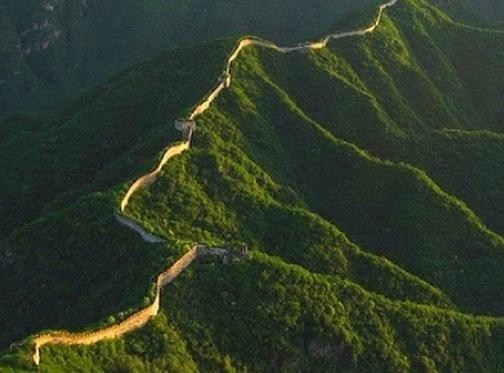
\includegraphics[scale=0.5]{great-wall}}
\end{frame}

\begin{frame}{Back to China again - border and access to information}
\centerline{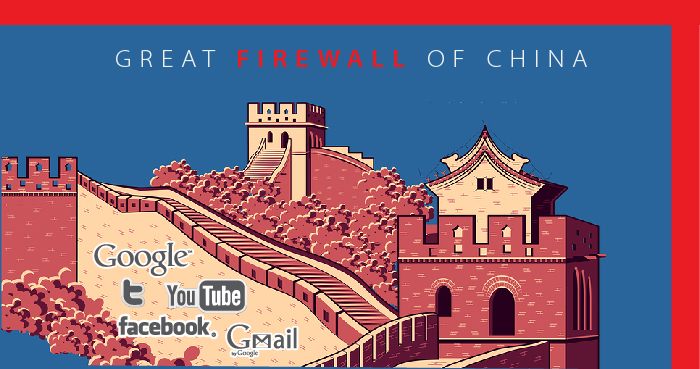
\includegraphics[scale=0.4]{firewall}}
\end{frame}
% what about poland?
% at least 3 organisation are legaly allowed to just block websites from the internet
% they're openly admiting that they're blocking gambling websites

% what is github?
% it is blocked from 2013
% they striked with 1.3Tb/s of traffic (highest rate of all time)
% north korea did the similar thing to SONY Pictures
\begin{frame}{Back to China again - firepower}
\centerline{\url{https://github.com/greatfire/wiki}}
\end{frame}

\begin{frame}{Back to China again - firepower}
\centerline{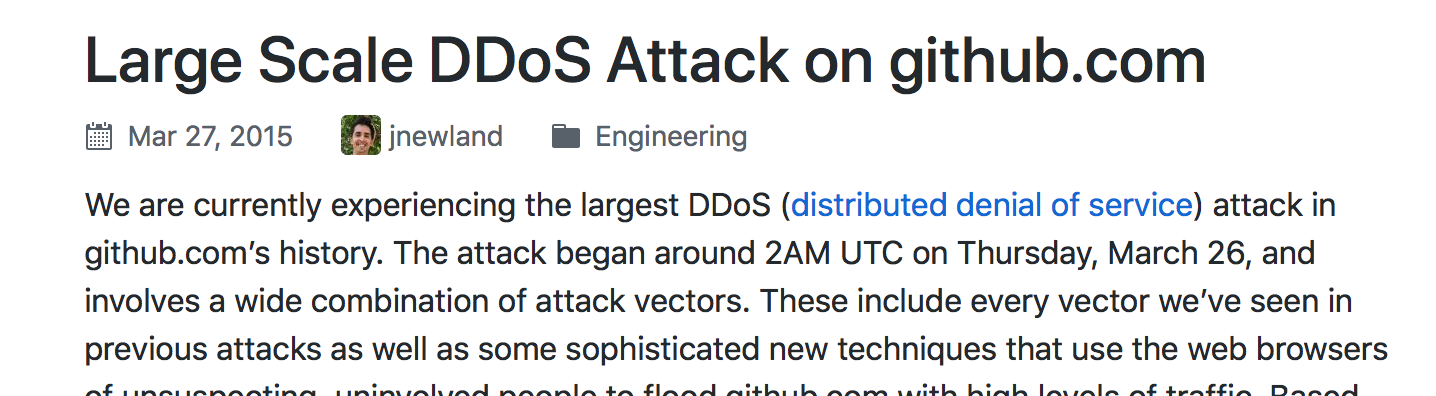
\includegraphics[scale=0.4]{gh2}}
\centerline{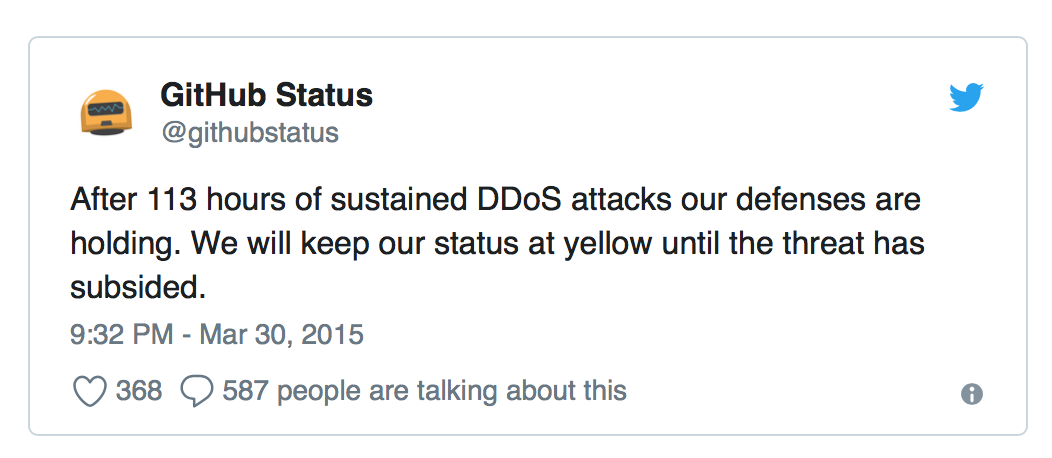
\includegraphics[scale=0.4]{gh1}}	
\end{frame}

\begin{frame}{}
\Large{I can’t change who you are but I have the power to choose my friends} \\
\vspace{0.5em}
\Large{One person’s Internet freedom is another’s Internet imperialism.} \\
\vspace{0.5em}
\Large{Join us in building up a peaceful, safe, and open and co-operative cyberspace.} \\
\vspace{0.5em}
\small{\textit{Lu Wei - Head of Internet Information Office}}
\end{frame}

% ----------------- Dominik Katszer ----------------
\section{The Sources of Cyber Power}
\begin{frame}{Cyber meaning}
\begin{itemize}
\item Definition\\
Term was introduced as a Greek transaltion which means governing or stering, however currently it has a lot of definitions depending on context.
\item Daily life\\
The internet is everywhere, everything is getting more smart and barier between offline and online life disappears
\end{itemize}
\end{frame}
\begin{frame}{Cyber layers}
\begin{itemize}
\item Hardware\\
Each hardware like e.g. router, cables gives a control of data flow through internet.
\item Software\\
Every kind of malware and even subsidizing operating systems and search engines like Google
\item Fake social account\\
It can be easily used for spreading disinformation. Nowadays it is hard to distiguish true facts from fake or blured news.
\end{itemize}
\end{frame}
\begin{frame}{Components of cyber power}
\begin{itemize}
\item Size
\item Shared mission and private sector
\item Adventurous and inventive military and intelligence agencies
\item Attractive narrative of cyberspace
\end{itemize}
\end{frame}
\begin{frame}{Size}
\Huge{How would your life look like without Google or Facebook ?}
\end{frame}
\begin{frame}{Size}
\begin{itemize}
\item The more hardware (phones, serwers, routers) state produce the better. It makes customer addicted to specific company or state.
\item Currently US dominates internet economy. 
\item Worth to remember that the more your country is active in the internet the more influence it exerts on foreign companies and governance.
\item sophisticated technology is also a source of vulnerability, everything can be a target of cyberattack.
\end{itemize}
\end{frame}
\begin{frame}{Size}
Example of hardware dominating:\newline \newline
Data passed via internet is mainly passed by US for example email from Brazil to Peru can be transported through California, so they can take advantage of this fact.
\end{frame}
\begin{frame}{Shared mission and private sector}
\textbf{Relationship between government and private sector}
\begin{itemize}
\item State secure technology company through law, money , idealogy etc
\item State can even cooperate with foreign parters and enforce some regulations abroad.  
\item In return they got antyviruses, technological development and data. 
\end{itemize}
\end{frame}
\begin{frame}{Shared mission and private sector}
“Surveillance is the business model of the Internet.” - Google, Facebook, Twitter collect personal data, mails etc. we think that everything is free but it is wrong, we pay with our personal data
 then they e.g .can personalize adverts .
 \newline \newline Nowadays most of companies try to collect as much data as possible , and this is the reason why big data field in computer sciencie is still growing up.
\end{frame}
\begin{frame}{Shared mission and private sector}
\textbf{~\newline National cybersecurity has to be a shared mission} - \textit{Barack Obama}\newline\newline
He said that because a lot of critical infrastructures are in private sector where he dont have direct access.
Government and private sector are interdependenced.
\newline\newline
If governance want to harness  the energy and innovation of the private sector then they are making business abroad.
\end{frame}
\begin{frame}{Military and intelligence agencies}
\begin{itemize}
\item Making real impact which does not only rely on breaking into machine, is not  easy.
\item US spends three to four times more on cyber offense than it does on defense.
\item What is more, the more intense the military competition, the more
rapid the innovation and development will be.
\end{itemize}
We don't have to look far for surveillance example. Facebook, Tweeter, FBI, CIA. Different between social media and organisations like CIA is about how they get data. In social media we give them freely.
\end{frame}
\begin{frame}{Military and intelligence agencies}
\Huge{How sophisticated surveillance or  cyberattack can be ?}
\end{frame}
\begin{frame}{Military and intelligence agencies}
Everything is possible if you have enough budget, time and specialists.\newline\newline
\textit{“any sufficiently advanced technology is indistinguishable from magic"} -- Arthur C. Clarke 
\end{frame}
\begin{frame}{Attractive narrative of cyberspace}
It is very important, because in that way government is convincing users to itself. \newline\newline
US : \newline
United States will work toward an “open,interoperable, secure, and reliable information and communications infrastructure.” which is a bit hypocritical because of how US is engaged in extensive surveillance.
US tryes to have one global network which can be controlled by them.
\end{frame}
\begin{frame}{Attractive narrative of cyberspace}
China: \newline
China is not of an open global platfrom but rather of one fragmented bynational jurisdictions and regulations.
They even use technology for inspection of internet content by checking send packages.
examines the content of the messages, scanning for sensitive key words and blocking access to sites
\newline\newline
Europe:\newline
Privacy as a fundamental right has translated into widely copied trade policies
and regulatory models. promote the protection of online rights. 
\end{frame}
\begin{frame}{True Cyber Superpowers}
\section{The True Cyber Superpowers}
\begin{itemize}
\item China and the United States are the only true cyber superpowers which managed to put all four of the building blocks together. 
\item Russia is almost there without one block. They lose the competition in producing technologies and services which are shaping cyberspace.
\item Other countries also are significant in the this field, however they are more restraint. 
\item There also exists states which citizens have doesnt have free access to the internet so surveillance is limited. Some countries also are not very well technologically developed so they are at the end of rate.
\end{itemize}
\end{frame}
\begin{frame}
\Huge{Which country has the best hackers ?}
\end{frame}

%----------------------------------KN dud----------------------------------------
\section{The New International Order}
\begin{frame}{Cyberspace usage motivations}
While Cyberspace is hard to compare to anything we've seen before, we can outline state's motivations:
\begin{itemize}
\item increase access to information and communication technologies to spark economic growth,
\item protect their own information assets and citizens...
\item but at the same time exploit and damage those of other countries,
\item access the data of their own citizens for intelligence and law enforcement.
\end{itemize}
% The Hacked World Order is emerging from the interactions of those powers
\end{frame}

\begin{frame}{Cyberspace usage classification}
Each state has a different road to reach its desires. \newline
Five fundamental questions determine the culture of country's user of cyber power,
how a nation-state:
\begin{enumerate}
\item interprets threats,
\item uses force,
\item exerts influence,
\item spurs innovation,
\item delineates the national good.
\end{enumerate}
% the anwsers delineate American, Chinese and Russian ways of cyber statecraft
\end{frame}

\begin{frame}{Internal and External Hazards}
\textbf{What is the balance between internal and external threats?} \newline
Both the liberal democracies and authoritarian states collect data to prevent terrorist attack (external),
but authoritarian regimes collect much more data about their own citizens.
\begin{itemize}
\item USA advocates for open internet, argumenting that societies get stronger the freer information flows,
\item China sees controlling information as a primary security concern,
\item Russia is trying to remove Western influence from the Web.
\end{itemize}

% the governments vaccum up as much data as possible
% Creativeness, accountability and competitiveness all gain with free internet
% the line is blurred seeing USA's invasion of their citizen's privacy
% democracies are also not free of censorship on the internet, 
% e.g. copyright violations on YT, piracy, extremist views result in blocking
% Russia claiming disinformation coming from the West, paranoid about USA
\end{frame}

\begin{frame}{Disruption and Destruction}
\textbf{How do you use force and military power in cyberspace?}
\begin{itemize}
\item what happens in cyberspace is mostly out of the sight of the public
\item offense in cyberspace is considered the best defense
\end{itemize}
The USA uses cyberattacks in two different ways:
\begin{itemize}
\item surgical and precise, like Stuxnet, requiring much preparation and military intelligence,
\item small attacks, like stealing data from a company, DDoS attack on country's banks.
\end{itemize}
% we don't know too much about cyberattacks, they are kept a secret
% smaller attacks are unlikely to provoke military action, but still serve political goals of harassment and undermining
\end{frame}

\begin{frame}{Space between}
\textit{``You have diplomacy, economic sanctions... and then you
have military action. In between there’s this space, right? In cyber,
there are a lot of things that you can do in that space between that can
help us accomplish the national interest.''} -- Eric Rosenbash, Assistant Secretary of Defence
% Russia exploits the in-between space much more freely than other states, e.g. Crimea
\end{frame}

\begin{frame}{Diplomats and Trolls}
\textbf{How to excert influence in the digital age?}
\begin{itemize}
\item digital age brought more public diplomacy,
\item ``war of narratives'' on social media, and on the internet in general,
\item flooding the internet with disinformation and propaganda.
\end{itemize}
% politicians on Twitter, Trump tweeting about Syria strike before it's been decided
% the point was to increase exposure to information, but we've become flooded with it
% speed over accuracy on social media, causing overflood with information
% russian trolls pushing their own agenda on all the corners of the internet (Twitter, Reddit, Facebook)
% some examples of russian trolls?
\end{frame}

\begin{frame}{Silicon Valley, Beijing and Brussels}
\Large{\textbf{What model of technological competition is best adapted for the future?}} \newline
Based on Sillicon Valley, Beijing and Brussels models
\end{frame}

\begin{frame}{Silicon Valley}
\begin{itemize}
\item innovation and entrepreneurship
\item highly focued on private sector
\item hoping on being the most competitive
\end{itemize}
% hoping on the private's market self-regulation
\end{frame}

\begin{frame}{Beijing}
\begin{itemize}
\item government controlling long-term goals
\item minimizing dependence on foreign technology
\end{itemize}
% especially not trusing USA (obvious after Snowden's thing)
% independence especially in all technology related to national security
\end{frame}

\begin{frame}{Brussels}
\begin{itemize}
\item more managerial than Silicon Valley, and less interventionalist than the Beijing one
\item protecting privacy, managing inequality, promoting social welfare
\item regulation to the market, using the gravity of the European market to shape technological trajectories.
\end{itemize}
%% obviously these are not hard-and-fast rules. 
% China has tried to recreate Silicon Valley locally, 
% Washington has blocked Chinese telecoms from domestic markets
\end{frame}


\begin{frame}{The social contract}
\textbf{What is the balance between individual rights and state interests in the digital age?}
\begin{itemize}
\item highly debated topic nowadays, with individual's right to privacy,
\item every society is confronting the question of what to do with the massive amounts of data,
\item in liberal democracies the access to data by the state is considerable, but limited,
\item authoritarian states mostly see their citizens data as tool to use for their advantage.
\end{itemize}
% massive amounts of data from the internet, cameras, sensors
% Authoritarian states mostly think about self preservation. Protecting their citizens from breaches, but also using the information about own's citizens for state preservation.
% Authoritarian states put high value on protecting their citizens data from outside attacks though
\end{frame}



% ----------------- CONCLUSION-------------------
\begin{frame}
% There is a lot of politics in digital world
% It's affecting a lot of areas such as economory or military
% Hacking attacks can target both countries and individual people
\frametitle{Conclusion}
\Huge{\centerline{Conclusion}}
\end{frame}

\end{document}